\setchapterpreamble[u]{\margintoc}
\chapter{Annual analysis: ANDASOL-II CSP plant}%CSP and inland-MED}
\labch{cc:simulation}

\tldrbox{
    This chapter presents the annual simulation results for different cooling
    systems: a \gls{wctLabel}, a \gls{dcLabel} and the presented \gls{ccLabel}
    optimized with static optimization and with horizon optimization. They
    provide cooling to the power block of the XX hours storage--\gls{cspLabel}
    plant ANDASOL-II with an off-peak operation strategy. Results for the case
    study report a specific cooling cost of XX, XX and XX for the
    \gls{wctLabel}, \gls{dcLabel} and \gls{ccLabel}, respectively, compared to
    the 5~L/kWh figure provided by the developer.
}

\section*{Introduction}
\addcontentsline{margintoc}{section}{Introduction}

\begin{marginfigure}[] % -5.5cm
    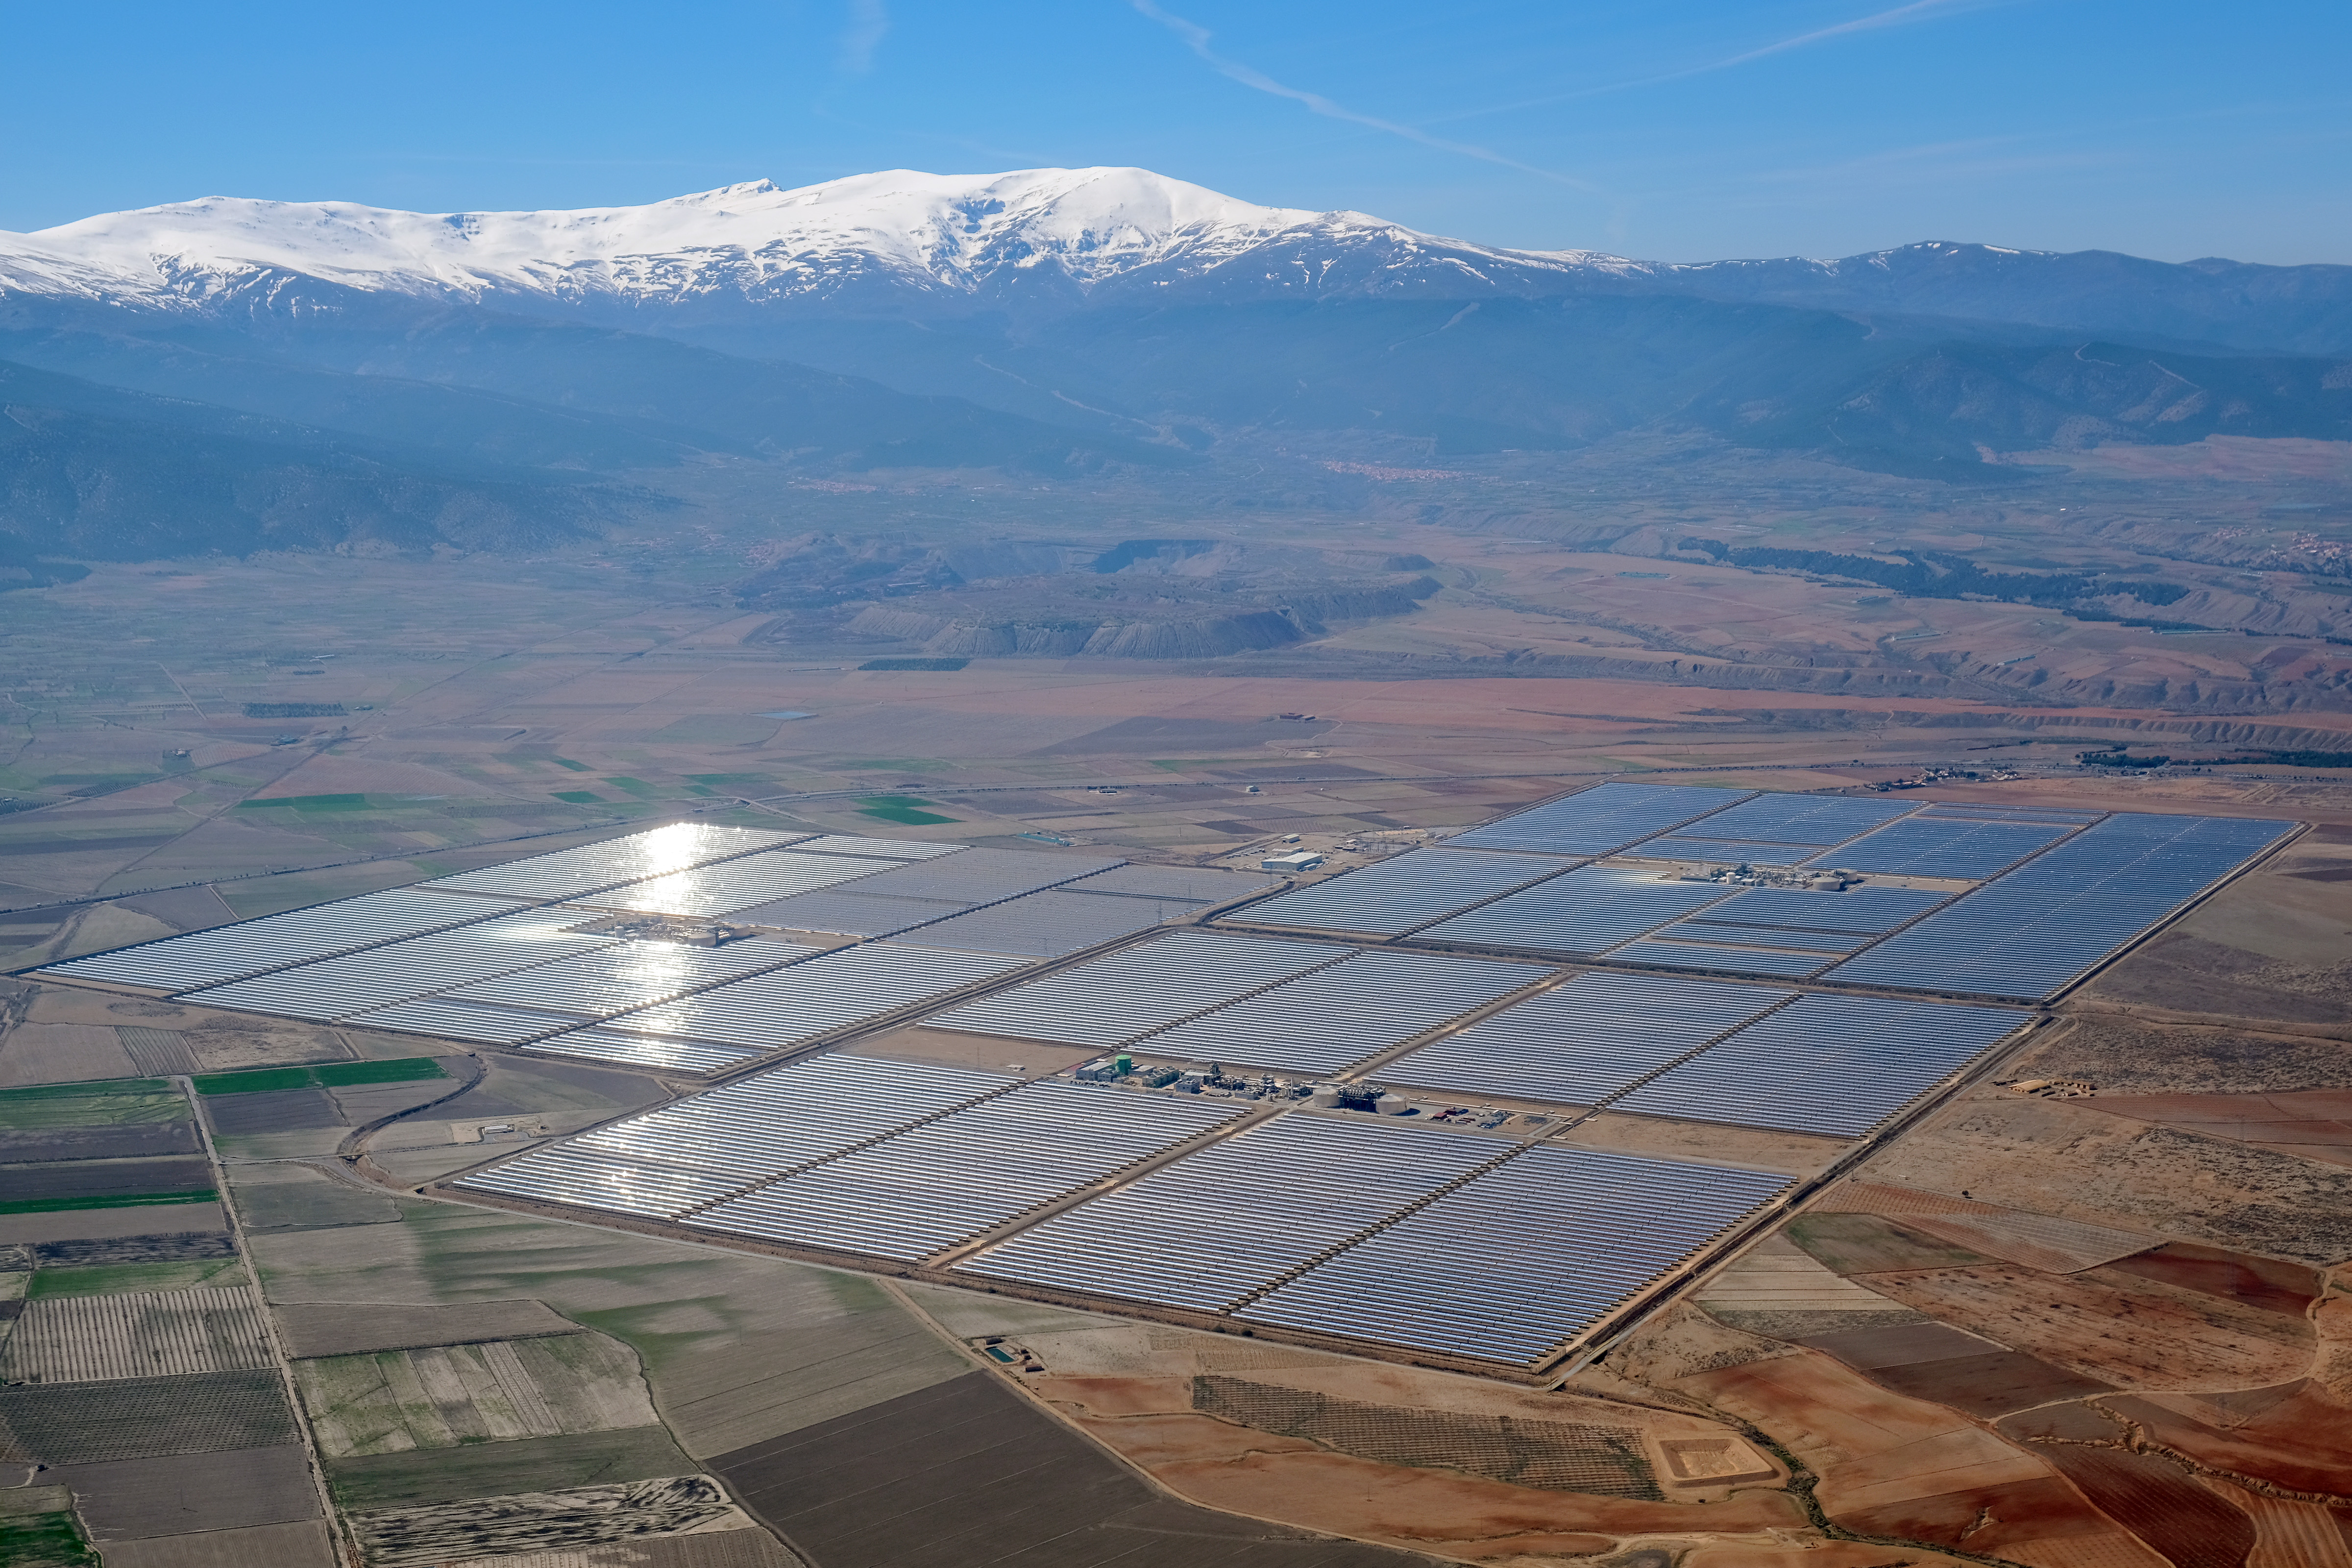
\includegraphics[]{figures/andasol.jpg}
    \caption[Andasol I, II and III]{Andasol I, II and III aerial view.
    Andasol-II is the one at .\\ 
	{\tiny Source: \url{https://en.wikipedia.org/wiki/File:Andasol_5.jpg}}}
    \labfig{cc:simulation:andasol}
\end{marginfigure}

% Introducción
A modeling framework has been developed to simulate and optimize the operation
of various cooling systems, with a particular focus on the proposed combined
cooling system. This methodology has been validated using data from a pilot
plant. In this chapter, the objective is to apply the framework to a specific
case study: a \fullgls{cspLabel} plant.

As previously mentioned, CSP plants are among the most water-intensive power
generation technologies~\sidecite[*2]{meldrum_life_2013}, a concern that is
especially relevant in the arid regions where they are typically located. To
assess the performance-water use and operational costs- of different cooling
systems, the proposed methodology is applied to a real-world case study through
an annual simulation. The case study examined is the Andasol-II \gls{cspLabel}
plant.

% Descripción ANDASOL
In the south-east of Spain, near Guadix and next to the Sierra Nevada mountain
range (see \reffig{cc:simulation:andasol}), thanks to the region high altitude
(1100~m) and the semi-arid climate, the site has exceptionally high annual
direct insolation (2260~W/m$^2$) and thus is ideal for solar projects. This is
why the first parabolic trough power plant in Europe, Andasol-I, was
built there in 2008. One year later Andasol-II followed, located in the immediate
neighbourhood and with almost identical construction. It has a rated output of
50~MW with 7.5~hours\sidenote[][]{This means that if fully charged, it can
produce the nominal rated power of the turbine for that duration} of thermal
storage, providing electricity for up to 200,000 people. More specifications
are available in \reftab{cc:simulation:andasol}.

According to the developer, Andasol-II vaporizes 870 000 m$^3$/year, or in
specific units \textbf{5 l/kWh}.

\begin{margintable}[*-3]
    \caption{ANDASOL-II plant main characteristics}
    \labtab{cc:simulation:andasol}
    \resizebox{\linewidth}{!}{
    \begin{tabular}{|l|l|}
        % \toprule
        % \textbf{Parameter} & \textbf{Value} \\
        % \midrule
        Technology & Parabolic Trough \\
        Solar Resource & 2260 W/m$^2$ \\
        Nominal Capacity & 50 MW \\
        Status & Operational \\
        Start Year & 2009 \\
        Expected Generation & 158 GWh/year \\
        Total Land Area & 2 km$^2$ \\
        LCOE (2020) & 0.27 €/kWh \\
        TF Inlet Temperature & 293$^\circ$C \\
        TF Outlet Temperature & 393$^\circ$C \\
        Power Cycle & Steam Rankine \\
        Turbine Efficiency & 38.1\% \\
        Cooling Type & Wet \\
        Storage Type & Molten salts \\
        Storage Capacity & 7.5 Hours – 1 GWh \\
        % \bottomrule
        % \multicolumn{2}{l}{} \\
    \end{tabular}
    \vspace{0.5em}
    }
    \scriptsize \textcolor{black!50!gray}{Source: Institute for Advanced Sustainability Studies (IASS) and others, 2022; data by Lilliestam@IASS, Thonig@IASS, Zang@CAS, Gilmanova@CAS and others. Licensed under a \href{https://creativecommons.org/licenses/by/4.0/}{Creative Commons Attribution 4.0 International License}.}
\end{margintable}

% Estructura del capítulo

%===================================
%===================================
\section{Limitations}
\labsec{cc:simulation:limitations}\todo{Considerar mover esto al apartado de
trabajos futuros}

\begin{enumerate}
    \item The combined cooler analyzed has a 50\% split in nominal cooling
    power of the \gls{wctLabel} and \gls{dcLabel} components compared to the
    standalone cooling systems. Different ratios could be analyzed and one
    would probably be a better fit for the particular case study. This in
    itself is a design optimization problem that is not addressed in this
    thesis.
    \item An \fullgls{acheLabel} is used for the \gls{dcLabel}, but other
    options could be considered, such as an \fullgls{accLabel}.
\end{enumerate}

%===================================
%===================================
\section{Environment definition}
\labsec{cc:simulation:environment}


%================================
\subsection{Water context}
\labsec{cc:simulation:environment:water}

Obtaining accurate water availability data is challenging. Unlike resources
such as electricity—where demand, supply, and prices are readily
available—water availability data is often lacking. Water prices are not
standardized; they vary from region to region, and even within the same region,
depending on the source and the specific agreements in place.

For the simulation scenario, two sources of water are considered\sidenote{See
\nrefsec{cc:fig:cc:optimization:environment}}. The first source is rainwater or
water from a dam, which is assumed to be available at a constant price of
XX~\sidecite{}. To create a representative dataset, water availability is
modeled as a function of precipitation data, which can be obtained from hourly
\gls{tpyLabel} data~\sidecite{meteonorm_}. A linear model is fitted to relate
maximum precipitation to maximum available water, and when there is no
precipitation, water availability is set to zero. The data is then resampled
every 15 days, and the daily volume of available water is calculated by
dividing the resampled fortnightly volume by 15. This approach accounts for the
presence of water reservoirs and some degree of management capacity.

The alternative source is regenerated water\sidenote{This is not an exogenous
idea; the Villena CSP plant, for example, uses wastewater from a nearby prison
to partially meet its water needs~\cite{}} is not limited in volume.

%================================
\subsection{Thermal load}
\labsec{cc:simulation:environment:load}

Traditionally, thermal power plants were designed and operated to generate
electricity only when solar energy was available. This approach remained common
until the rapid rise in competitiveness of \gls{pvLabel} plants, which offer
significantly lower generation costs. In response, concentrated solar power
plants began integrating thermal energy storage systems to enable dispatchable
power generation. Today, 21 out of 51 CSP plants in Spain—approximately
42\%—have thermal storage capacities exceeding two
hours~\sidecite{thonig_cspguru_2023,lilliestam_midterm_2021,bonilla_csp_2024}.
This enables them to produce electricity even when solar input is unavailable.

However, many of these plants still follow traditional operating patterns,
generating most of their electricity during peak solar hours\sidenote{The
storage is primarily used to extend generation past sunset.}. This strategy is
increasingly seen as suboptimal and is likely to be phased out as the electric
grid becomes saturated with \gls{pvLabel} generation\sidenote{This trend is
already observable in Spain during the summer months; see
\reffig{cc:simulation:mix}}.

% Poner figura de presentación con datos de REE
\begin{figure}
    \includegraphics[width=\textwidth]{figures/spanish-electric-mix-20240712.png}
    \caption{Spanish electricity mix on July 12, 2024. The peak in
    photovoltaic generation is clearly visible at midday, while thermosolar
    generation is more evenly distributed throughout the day. Peak production
    is majorly from CSP plants with no storage.\\
    {\scriptsize \textcolor{black!50!gray}{Data source: Figure elaborated using data
    extracted from \url{https://www.ree.es/es/datos}}}}
    \labfig{cc:simulation:mix}
\end{figure}


In this work, a different operational strategy is adopted: the plant is
configured to generate electricity during off-peak solar hours, typically in
the evening when electricity demand is at its highest. This is achieved by
shifting the plant’s production to align with these peak demand periods.

A model of the Andasol-II plant, developed by Bartolomé et al.~\sidecite{}, was
configured to follow this production strategy and simulated over an entire
year. The resulting thermal load profile represents the demand to be met by the
cooling system. The simulation used the same weather dataset as that employed
for modeling the cooling system.


%================================
\subsection{Costs context}
\labsec{cc:simulation:environment:costs}

\textbf{Electricity}. The spanish grid operator \gls{reeLabel} provides an API\sidenote{
    \qrcode[hyperlink,height=0.5in]{https://api.esios.ree.es}\\ \href{https://api.esios.ree.es}{https://api.esios.ree.es}
} to access the electricity market prices. A python script was developed to
systematically download monthly data\sidenote{Longer periods would result in
silent errors in the API} for each month in the desired year. The data is
fetched in hourly intervals and saved in JSON format, then every file is
read and joined into a single dataset resulting in prices for the whole year. 

\textbf{Water}. Rainwater has a constant lower price of XX. This price was
obtained considering that the plan has access to the same water than the
irrigation community of the area\sidecite{}. The alternative source, \ie
regenerated water, is considerably more expensive, and its price is linked to
the electricity price, specifically by a factor of XX\sidenote{This value
includes a scaling factor to normalize the values}.

\begin{kaobox}[title=Simulation data and parameters information] 
    \begin{itemize}
        \item[Weather data] Hourly weather data from \gls{tpyLabel} of
        Guadix (Spain) for the year. Data was obtained from ...
        \item[Thermal load] Hourly thermal load data from the power block
        of ANDASOL-II CSP plant from a simulation model.
        \item[Electricity price] Spanish electricity market from 2022.
        \item[Maximum available water] The maximum available water for ...
        \item[Alternative water source factor] ...
    \end{itemize}
    
    \begin{tabular}{p{0.3\textwidth} c} 
        The full environment dataset is available at  &
        \qrcode[hyperlink,height=0.5in]{\solhycoolRepositoryBaseUrl/data/datasets/environment_data_andasol_20220101_20241231.csv}
    \end{tabular}
\end{kaobox}

% \section{WCT results}
% Anual muestreado cada 15 días. Versión interactiva sin muestrar
% \begin{figure}
%     \includegraphics[width=1.2\textwidth]{figures/cc-simulation-wct-year_viz_resampled.png}
%     \savebox\captionqr{\qrcode[hyperlink,height=0.5in]{\repositoryBaseUrl/figures/cc-simulation-wct-year_viz.html}}
%     \caption{Annual simulation results for the \gls{ccLabel} system optimized
%     with static optimization. Results are resampled every 15 days using their
%     mean values. The original frequency results can be found in the interactive
%     version:\\[1ex] \usebox\captionqr}
%     \labfig{cc:simulation:wct-year}
% \end{figure}

% \section{DC results}
% \begin{figure}
%     \includegraphics[width=1.2\textwidth]{figures/cc-simulation-dc-year_viz_resampled.png}
%     \savebox\captionqr{\qrcode[hyperlink,height=0.5in]{\repositoryBaseUrl/figures/cc-simulation-dc-year_viz.html}}
%     \caption{Annual simulation results for the \gls{ccLabel} system optimized
%     with static optimization. Results are resampled every 15 days using their
%     mean values. The original frequency results can be found in the interactive
%     version:\\[1ex] \usebox\captionqr}
%     \labfig{cc:simulation:dc-year}
% \end{figure}


% \section{CC results}
% \subsection{Static optimization}

% \begin{figure}
%     \includegraphics[width=1.2\textwidth]{figures/cc-simulation-cc_static-year_viz_resampled.png}
%     \savebox\captionqr{\qrcode[hyperlink,height=0.5in]{\repositoryBaseUrl/figures/cc-simulation-cc_static-year_viz.html}}
%     \caption{Annual simulation results for the \gls{ccLabel} system optimized
%     with static optimization. Results are resampled every 15 days using their
%     mean values. The original frequency results can be found in the interactive
%     version:\\[1ex] \usebox\captionqr}
%     \labfig{cc:simulation:cc-static-year}
% \end{figure}




% \subsection{Horizon optimization}


% 1 day en detalle (incluya frente de pareto, compare distribución hidráulica y
% tenga el coste acumulado comparado)

% Annual results
% \begin{figure}
%     \includegraphics[width=1.2\textwidth]{figures/cc-simulation-cc_static-year_viz_resampled.png}
%     \savebox\captionqr{\qrcode[hyperlink,height=0.5in]{\repositoryBaseUrl/figures/cc-simulation-cc_static-year_viz.html}}
%     \caption{Annual simulation results for the \gls{ccLabel} system optimized
%     with static optimization. Results are resampled every 15 days using their
%     mean values. The original frequency results can be found in the interactive
%     version:\\[1ex] \usebox\captionqr}
%     \labfig{cc:simulation:cc-static-year}
% \end{figure}


%================================
\section{Optimization strategies comparison}[Comparison]
\labsec{cc:simulation:optimization-comparison}

% 3 in 1 cc-static
% {\newgeometry{margin=0.5cm}  % Remove margins completely

% \begin{sidewaysfigure*}
%     \centering
%     \includegraphics[width=.9\paperheight, keepaspectratio]{figures/test.png}
%     \caption{A rotated figure}
% \end{sidewaysfigure*}

% \restoregeometry}


% % 3 in 1 cc-horizon
% % TODO: añadir cumulative costs comparison
% {\newgeometry{margin=0.5cm}  % Remove margins completely

% \begin{sidewaysfigure*}
%     \centering
%     \includegraphics[width=.9\paperheight, keepaspectratio]{figures/test.png}
%     \caption{A rotated figure}
% \end{sidewaysfigure*}

% \restoregeometry}

% 3 in 1 cc-static
{%
\newgeometry{margin=0.5cm}
\begin{figure}
    \savebox\captionqr{\qrcode[hyperlink,height=1cm]{\repositoryBaseUrl/figures/test.html}}
    \caption{\gls{ccLabel} static optimization simulation results in three
    different periods of time \hspace{1ex}\usebox\captionqr}
    \makebox[\textwidth][c]{\includegraphics[angle=90,width=0.9\paperwidth]{temp/test.png}}%
\end{figure}%
\restoregeometry
}

% 3 in 1 cc-horizon
{%
\newgeometry{margin=0.5cm}
\begin{figure}
    \savebox\captionqr{\qrcode[hyperlink,height=1cm]{\repositoryBaseUrl/figures/test.html}}
    \caption{A rotated figure \hspace{1ex}\usebox\captionqr}
    \makebox[\textwidth][c]{\includegraphics[angle=90,width=0.9\paperwidth]{temp/test.png}}%
\end{figure}%
\restoregeometry
}


\section{Cooling alternatives comparison}
\labsec{cc:simulation:alternatives-comparison}

% \begin{figure*}[h!]
%     \includegraphics[]{figures/.png}
%     \savebox\captionqr{\qrcode[hyperlink,height=0.5in]{\repositoryBaseUrl/figures/.html}}
%     \caption[Figure caption]{Figure caption.\hspace{1ex}\usebox\captionqr}
%     \labfig{::}
%         \end{figure*}
Fusionar las gŕacias de resultados anuales remuestreados para que incluyan
todas las alternativas. Cambiar fondo para cada sistema
\begin{figure*}[h!]
    \includegraphics[width=1\linewidth]{figures/year_viz_comp_SME-15.png}
    \savebox\captionqr{\qrcode[hyperlink,height=0.5in]{\repositoryBaseUrl/figures/year_viz_comp_SME-15.html}}
    \caption{Annual simulation results for the \gls{ccLabel} system optimized
    with static optimization. Results are resampled every 15 days using their
    mean values. The original frequency results can be found in the interactive
    version:\\[1ex] \usebox\captionqr}
    \labfig{cc:simulation:year-comparison}
\end{figure*}


\todo{Añadir gráfica de barras comparando coste por kWh refrigerado}
\todo{Añadir gráfica de barras comparando distribución de potencia térmica por componente
y distribución hidráulica por componente para cc-static y cc-horizon}
% Apoyarse también en las trazas de comparación que se añaden en las gráficas
% de la versión con horizonte

